\section{Description and Methodology}

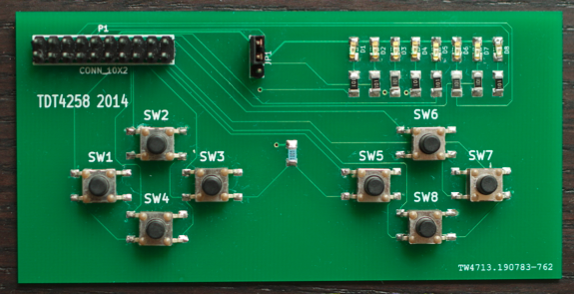
\includegraphics{figures/gamepad.png}
This report describes three distinct systems; Each one more more power efficient than the last.

The first implementation is a simple polling-based approach. The second one uses interrupts, removing time needlessly used for idling. The final system goes into a deep sleep mode, waking only when coerced to do so by an interrupt from the GPIO controller.

Energy consumption was noted for each improvement to the system, and one can clearly see how power consumption is reduced by multiple orders of magnitude in the final system.

\subsection{A program without interrupts}

The first system implements a simple polling-based mechanism for updating the LEDs on the gamepad. The main loop simply loads whatever values are found on the gamepad (GPIO port C, pins 0-7), shifts them to the appropriate position required by the output port (GPIO port A, pins 8 - 15), and sets the corresponding pins to logical low.

\subsection{A program with interrupts}

The second system contains a simple, yet important architectural change. The system no longer blindly loads register values form input to output, instead only updating them when interrupts are received from the gamepad.

External interrupt generation for GPIO port C is now allowed. , as well as edge-driven in
Edge-driven interrputs are enabled for transitions from both high to low, as well as low to high.

\begin{lstlisting}
\end{lstlisting}


\subsection{A program using low energy modes}
